\chapter{Model-Based Reinforcement Learning}
What we have covered so far can be categorized as ``model-free'' reinforcement learning. The reason why it is called model-free is that the transition probabilities are unknown and we did not even attempt to learn the transition probabilities. Recall the RL objective:
\begin{align*}
  \pi_\theta(\tau) &= p_\theta(s_1,a_1,...,s_T,a_t)\\
  &= p(s_1)\prod_{t=1}^T\pi_\theta(a_t|s_t)p(s_{t+1}|s_t,a_t)\\
  \theta^* &= \argmaxA_\theta\mathbb{E}_{\tau\sim p_\theta(\tau)}\left[\sum_t r(s_t,a_t)\right]
\end{align*}
The transition probabilities $p(s_{t+1}|s_t,a_t)$ is not known in all the model-free RL algorithms that we have learned such as Q-learning and policy gradients. But what if we know the transition dynamics? Recall that at the very beginning of the notes we drew an analogy of RL and control theory; in many cases, we do know the system's internal transition. For example, in games, easily modeled systems, and simulated environments, the transitions are given to us. Moreover, it is not uncommon to learn the transition models: in classic robotics, system identification fits unknown parameters of a known model to learn how the system evolves, and one could also imagine a deep learning approach where we could potentially fit a general-purpose model to observed transition data for later use. In fact, the latter case is the essence of Model-based RL, where we learn the transition dynamics first, and then figure out how to choose actions. To learn about model-based RL, we shall start from a simpler case, where we know the transitions and determine how we control the system optimally based on the transitions. After this, we can apply our optimal control theory to the more general case, where we actually learn the transitions first.
\section{Optimal Control}
Optimal control is a task that we come across when we are well aware of the transition probabilities and we try to learn how to control the system optimally. In optimal control, there are two different categories of controller design: the first one is \textbf{open-loop} control, where we do not have any state feedbacks, and we roll out a sequence of actions based on the current state that we observe. The second one is called \textbf{closed-loop} control, where we determine the action at each time step based on the current state, and how we determine the action to apply is based on state feedbacks. In some cases, our transition functions are deterministic, while in others, the transition functions are stochastic.

In a open loop controller, if we have a deterministic transition in our system such that $a_{t+1} = f(s_t,a_t)$, then our action sequence should be determined by choosing those that can return the maximum rewards:
\begin{align*}
    a_1, ..., a_T&=\argmaxA_{a1...a_T}\sum_{t=1}^Tr(s_t,a_t)\\
    \mathrm{s.t. }\;a_{t+1} &= f(s_t,a_t)
\end{align*}
In stochastic scenarios, the transition function is a probabilistic distribution, where we have $p(s_{t+1}|s_t,a_t)$, and the action sequence should be chosen based on expectation of the rewards:
\begin{align*}
    p_\theta(s_1,...,s_T)&=p(s_1)\prod_{t=1}^Tp(s_{t+1}|s_t,a_t)\\
    a_1,...,a_T &= \argmaxA_{a_1,...,a_T}\mathbb{E}\left[\sum_t r(s_t,a_t)|a_1,...,a_T\right]
\end{align*}
Note that we roll out all actions to apply only based on the initial state marginal, so we do not consider any state-feedback in this case.

In a closed-loop controller, however, we keep interacting with the world, so we need a policy function that can tell us the action to apply if we input the current state: $a_t\sim \pi(a_t|s_t)$, which we call a state-feedback. We choose our policy function as follows:
\begin{align*}
    p(s_1,a_1,...,s_T,a_T) &= p(s_1)\prod_{t=1}^T\pi(a_t|s_t)p(s_{t+1}|s_t,a_t)\\
    \pi &=\argmaxA_\pi \mathbb{E}_{\tau\sim p(\tau)}\left[\sum_t r(s_t,a_t)\right]
\end{align*}
Generally, $\pi$ could take many forms, such as a neural net or time-variant linear controller $K_ts_t + k_t$.

\section{Open-loop Planning}
For now, let us focus on a simple, open-loop controller, and see how we choose actions using such controller. In open-loop scenarios, we roll out a sequence of actions by doing $\argmaxA$ on the sum of rewards:
$a_1,...,a_T = \argmaxA_{a_1,...,a_T}J(a_1,...,a_T)$
and compactly, we can say that $A = \argmaxA_A J(A)$.
\subsection{Random Shooting}
Perhaps the easiest and most intuitive stochastic optimization method in open-loop control is the random shooting method. In such method, we first sample some different action sequences $A_1,...,A_N$ from some known distribution (such as uniform), and then we choose $A_i$ based on $\argmaxA_i J(A_i)$. This is highly efficient in that we are not improving what we sample, so we might get stuck in some mediocre action sequence. Therefore, we can keep improving the samples we choose from a Gaussian distribution based on some elites sequences. This is the basic idea of Cross Entropy Method (CEM).

\subsection{Cross Entropy Method}
CEM improves upon the random shooting's guess and check scheme by choosing some elites sequences which give us higher rewards and refit the distribution to the high rewards. Intuitively, we are getting closer to higher rewards as we refit the distribution. Here is a sketch of CEM, as shown in Alg. \ref{alg:cem}.
\begin{algorithm}[t!]
\caption{Cross Entropy Method with Continuous-valued Input}
\begin{algorithmic}[1]
\label{alg:cem}
\REQUIRE Some base distribution for action sequence $p(A)$ 
\WHILE{true}
    \STATE Sample $A_1,...,A_N$ from $p(A)$
    \STATE Evaluate $J(A_1),...,J(A_N)$
    \STATE Pick elites $A_{i_1},...,A_{i_M}$ with the highest value, where $M<N$
    \STATE Refit $p(A)$ to elites $A_{i_1},...,A_{i_M}$
\ENDWHILE
\end{algorithmic}
\end{algorithm}
This algorithm is extremely simple and very fast if parallelized. However, it suffers from very harsh dimensionality limit and it only works for open-loop scenarios. 
\subsection{Monte Carlo Tree Search}
Now imagine our action space is discrete, we can apply a stochastic optimization technique called Monte Carlo Tree Search (MCTS), which is very popular in planning in stochastic games. The gist of this method is that in discrete action space, we are essentially expanding out a tree. However, the tree might be too big to expand out due to computational cost. Therefore, one way to save the computational cost is to partially expand the tree and use a policy to simulate a trajectory from the last expanded node. A generic sketch of MCTS is shown in Alg. \ref{alg:mcts}.
\begin{algorithm}[t!]
\caption{Generic Monte Carlo Tree Search (MCTS)}
\begin{algorithmic}[1]
\label{alg:mcts}
\REQUIRE Some base tree policy for expanding nodes, some base default policy to simulate a trajectory from a leaf
\WHILE{true}
    \STATE Find a leaf $s_l$ using TreePolicy($s_1$)
    \STATE Evaluate the leaf using DefaultPolicy($s_l$)
    \STATE Update all values in tree between $s_1$ and $s_l$
\ENDWHILE
Take best action from $s_1$
\end{algorithmic}
\end{algorithm}
Note that we the tree policy is not an actual policy, because it is just a method to traverse through our tree in order to select a node to expand. The default policy is an actual policy that is able to simulate the system. Since simulations are involved here, we have to be able to roll back to the original state.
\subsection{UCT Tree Policy}

In MCTS, how do we choose the nodes to expand? Intuitively, we need to keep choosing the nodes with high rewards so far, and simultaneously pick the ones that have not been chosen in order to explore. Therefore, one way to do it is to use the UCT tree policy. In this policy, we gauge the performance of each node by assigning a score function where Score$(s_t) = \frac{Q(s_t)}{N(s_t)}+2C\sqrt{\frac{2\ln{N(s_{t-1})}}{N(s_t)}}$. If the current node $s_t$ is not fully expanded, meaning that there is action that we never took before, then we choose new $a_t$; else, we choose the child with best Score($s_{t+1}$).

More details about MCTS can be found in \cite{browne2012survey} and \cite{guo2014deep}.

\subsection{Using Derivatives}
Let us consider the control theory counterpart of the RL objective. Essentially, we have a constrained optimization problem defined as follows:
$$\min_{u_1,...,u_T}\sum_{t=1}^Tc(x_t,u_t)\;\mathrm{s.t.}\;x_t = f(x_{t-1}, u_{t-1})$$
if we plug in the transition constraint, we have:
$$\min_{u_1,...,u_T}c(x_1,u_1) + c(f(x_1,u_1),u_2)+...+c(f(f(...)...),u_T)$$
which becomes an unconstrained optimization problem. Since it is unconstrained now, one might ask, can we do gradient descent on it? The usual answer is yes, but only if we use some more powerful optimization technique such as 2nd-order Newton method. Because optimization problems such as shooting methods are hard and often ill-conditioned via 1st order gradient descent. 
\subsection{Shooting Methods and Collocation Methods}
There are two different classes of gradient descent based method: shooting method and collocation method. In shooting methods, we optimize only on action sequences, so the actions are the only optimization variables. We only optimize upon the actions and apply the action to the state and see where it shoots to, so the states are the consequences of the actions that we optimize. The optimization problem can be written as:
$$\min_{u_1,...,u_T}c(x_1,u_1) + c(f(x_1,u_1),u_2)+...+c(f(f(...)...),u_T)$$

However, in collocation method, we optimize upon both actions and states, with constraints, and the optimization problem is written as:
$$\min_{u_1,...,u_T,x_1,...,x_T}\sum_{t=1}^Tc(x_t,u_t)\;\mathrm{s.t.}\;x_t = f(x_{t-1}, u_{t-1})$$

\subsection{Linear Quadratic Regulator (LQR)}
Let us start with a simple case of shooting method, where we apply a 2nd order-style optimization technique to achieve optimal control. The simple case assumes that we have a linear system, where the transition function is affine, and we have a quadratic cost function. 

Thus, the transition function should be of the form:
\[
f(x_t,u_t) = F_t \begin{bmatrix} x_t\\u_t\end{bmatrix}+f_t
\]
and the cost function should be of the form:
\[
c(x_t,u_t) = \frac{1}{2}\begin{bmatrix}x_t\\u_t\end{bmatrix}^TC_t\begin{bmatrix}x_t\\u_t\end{bmatrix}+\begin{bmatrix}x_t\\u_t\end{bmatrix}^Tc_t
\]
What we are doing right now is to solve for a closed-form solution for an optimal LQR controller. The idea is to use backward recursion. Since we are doing shooting method, we have $$\min_{u_1,...,u_T}c(x_1,u_1) + c(f(x_1,u_1),u_2)+...+c(f(f(...)...),u_T)$$
and the last item is the only term that depends on $u_T$. Therefore, as a base case, we can try to solve for $u_T$ first. In order to simplify our computation, let us define some blocks in the matrices that we defined above. Specifically, let us assume that
\[
C_T = \begin{bmatrix} C_{x_T,x_T}& C_{x_T,u_T}\\C_{u_t,x_T}&C_{u_T,u_T}\end{bmatrix}
\]
and
\[
c_T=\begin{bmatrix}c_{x_T}\\c_{u_T}\end{bmatrix}
\]

Since our cost function is
\[
Q(x_T,u_T) = \mathrm{const} + \frac{1}{2}\begin{bmatrix}x_T\\u_T\end{bmatrix}^TC_T\begin{bmatrix}x_T\\u_T\end{bmatrix}+\begin{bmatrix}x_T\\u_T\end{bmatrix}^Tc_T
\]
by setting gradient to 0, we will have 
\[
\nabla_{u_T}Q(x_T,u_T) = C_{u_t,x_T}x_T+C_{u_T,u_T}u_T+c_{u_T}^T=0
\]
By solving this equation, we have solved $u_T$, in terms of known constants and $x_T$:
\[
u_T = -C_{u_T,u_T}^{-1}(C_{u_t,x_T}x_T+c_{u_T})
\]
and to make notations more compact, let us denote $u_T$ as $u_T = K_Tx_T+k_T$, and $K_T = -C_{u_T,u_T}^{-1}C_{u_t,x_T}$, $k_T = -C_{u_T,u_T}^{-1}c_{u_T}$.

Now having solved our terminal control input $u_T$, which is fully determined by our terminal state $x_T$, we can eliminate $u_T$ in $Q(x_T,u_T).$ Plugging in, we have
\begin{align*}
V(x_T) &= \mathrm{const} + \frac{1}{2}\begin{bmatrix}x_T\\K_Tx_T+k_T\end{bmatrix}^TC_T\begin{bmatrix}x_T\\K_Tx_T+k_T\end{bmatrix}+\begin{bmatrix}x_T\\K_Tx_T+k_T\end{bmatrix}^Tc_T\\
&=\frac{1}{2}x_T^TC_{x_T,x_T}x_T + \frac{1}{2}x_T^TC_{x_T,u_T}K_Tx_T+ \frac{1}{2}x_T^TK_T^TC_{u_T,x_T}x_T + \frac{1}{2}x_T^TK_T^TC_{u_T,u_T}K_Tx_T\\& \phantomrel{=} {}  + x_T^TK_T^TC_{u_T,u_T}k_T + \frac{1}{2}x_T^TC_{x_T,u_T}k_T + x_T^Tc_{x_T} + x_T^TK_T^Tc_{u_T} + \mathrm{const}\\
&= \text{const} + \frac{1}{2}x_T^TV_Tx_T + x_T^Tv_T
\end{align*}
where we define $v_T$ and $V_T$ to make the notation more compact as follows:
\begin{align*}
    V_T &= C_{x_T,x_T} + C_{x_T,u_T}K_T +K_T^TC_{u_T,x_T} + K_T^TC_{u_T,u_T}K_T^T\\
    v_T&= c_{x_T} + C_{x_T,u_T}k_T+K_T^Tc_{u_T} + K_T^TC_{u_T,u_T}k_T
\end{align*}

Having solved the base case, we solve solve for other optimal control inputs backwards. Let us first proceed to solve for $u_{T-1}$ in terms of $x_{T-1}$. Now note that $u_{T-1}$ not only affects state $x_{T-1}$, but it also affects $x_T$ because of the system dynamics:
\[
f(x_{T-1}, u_{T-1}) = x_T = F_{T-1}\begin{bmatrix}x_{T-1}\\u_{T-1}\end{bmatrix} + f_{T-1}
\]
Therefore, the cost function from $T-1$ can be calculated as:
\[
Q(x_{T-1}, u_{T-1}) = \text{const} + \frac{1}{2}\begin{bmatrix}x_{T-1}\\u_{T-1}\end{bmatrix}^TC_{T-1}\begin{bmatrix}x_{T-1}\\u_{T-1}\end{bmatrix} + \begin{bmatrix}x_{T-1}\\u_{T-1}\end{bmatrix}^Tc_{T-1} + V(f(x_{T-1}, u_{T-1}))
\]
and if we plug the transition dynamics function into $V(x_T)$, we will have:
\[
V(x_T) = \text{const} + \frac{1}{2}\begin{bmatrix}x_{T-1}\\u_{T-1}\end{bmatrix}^TF_{T-1}^TV_TF_{T-1}\begin{bmatrix}x_{T-1}\\u_{T-1}\end{bmatrix} + \begin{bmatrix}x_{T-1}\\u_{T-1}\end{bmatrix}^TF_{T-1}^TV_Tf_{T-1}+\begin{bmatrix}x_{T-1}\\u_{T-1}\end{bmatrix}^TF_{T-1}^Tv_T
\]
More compactly, we write the cost function as:
\[
Q(x_{T-1}, u_{T-1}) = \text{const} +\frac{1}{2} \begin{bmatrix}x_{T-1}\\u_{T-1}\end{bmatrix}Q_{T-1}\begin{bmatrix}x_{T-1}\\u_{T-1}\end{bmatrix} + \begin{bmatrix}x_{T-1}\\u_{T-1}\end{bmatrix}^Tq_{T-1}
\]
where $Q_{T-1} = C_{T-1} + F^T_{T-1}V_TF_{T-1}$, and $q_{T-1} = c_{T-1} +  F^T_{T-1}V_Tf_{T-1} + F^T_{T-1}v_T$. To solve the optimization problem, we set the gradient to 0:
\[
\nabla_{u_{T-1}}Q(x_{T-1}, u_{T-1}) Q_{u_{T-1},x_{T-1}}x_{T-1} + Q_{u_{T-1},u_{T-1}}u_{T-1}+q_{u_{T-1}}^T=0
\]
solving the equation, we have the following expression for $u_{T-1}$:
\begin{align*}
    u_{T-1} &= K_{T-1}x_{T-1} + k_{T-1}\\
    K_{T-1} &= -Q^{-1}_{u_{T-1},u_{T-1}}Q_{u_{T-1},x_{T-1}}\\
    k_{T-1} &= -Q_{u_{T-1},u_{T-1}}q_{u_{T-1}}
\end{align*}

Applying the same technique backwards, we can solve for the states and inputs at each time step, as illustrated in Alg. \ref{alg:lqr}.
\begin{algorithm}[t!]
\caption{Solving for Linear Quadratic Regulator (LQR)}
\begin{algorithmic}[1]
\label{alg:lqr}
\STATE Backward Recursion
\FOR{$t = T$ to 1}
    \STATE $Q_t = C_t + F_t^TV_{t+1}F_t$
    \STATE $q_{t} = c_{t} +  F^T_{t}V_Tf_{t} + F^T_{t}v_{t+1}$
    \STATE $Q(x_{t}, u_{t}) = \text{const} +\frac{1}{2} \begin{bmatrix}x_{t}\\u_{t}\end{bmatrix}Q_{t}\begin{bmatrix}x_{t}\\u_{t}\end{bmatrix} + \begin{bmatrix}x_{t}\\u_{t}\end{bmatrix}^Tq_{t}$
    \STATE $u_t\leftarrow \argminA_{u_t}Q(x_t,u_t) = K_tx_t + k_t$
    \STATE $K_{t} &= -Q^{-1}_{u_{t},u_{t}}Q_{u_{t},x_{t}}$
    \STATE $k_{t} &= -Q_{u_{t},u_{t}}q_{u_{t}}$
    \STATE $V_t = Q_{x_t,x_t} + Q_{x_t,u_t}K_t + K^T_tQ_{u_t,x_t} + K_t^TQ_{u_t,u_t}K_t$
    \STATE $v_t = q_{x_t} + Q_{x_t,u_t}k_t + K_t^TQ_{u_t} + K^T_tQ_{u_t,u_t}k_t$
    \STATE $V(x_t) = \text{const} + \frac{1}{2}x_t^TV_tx_t + x_t^Tv_t$
\ENDFOR
\STATE Forward Recursion
\FOR{$t=1$ to T}
    \STATE $u_t = K_tx_t + k_t$
    \STATE $x_{t+1} = f(x_t,u_t)$
\ENDFOR
\end{algorithmic}
\end{algorithm}
In step 5 of Alg. \ref{alg:lqr}, Q-function represents the total cost from now until end if we take $u_t$ from state $x_t$, and in step 11, the V-function represents the total cost from now until end from state $x_t$, so $V(x_t) = \min_{u_t}Q_{x_t,u_t}$, which we call the cost-to-go function. 

What we have analyzed above is based on deterministic dynamics. What if the transition (dynamics) is stochastic? Specifically, consider the following setup:
\begin{align*}
    x_{t+1} &\sim p(x_{t+1}|x_t,u_t)\\
    p(x_{t+1}|x_t,u_t) &= \mathcal{N}\left(F_t\begin{bmatrix}x_t\\u_t\end{bmatrix} + f_t, \Sigma_t\right)
\end{align*}
where our transition is actually a Gaussian distribution with constant covariance. It turns out that we can apply the exact same algorithm, choosing actions according to $u_t = K_tx_t + k_t$, and we can ignore $\Sigma_t$ due to symmetry of Gaussians.

\subsection{Iterative LQR (iLQR)}
In LQR, we assumed that the dynamics are linear. In non-linear cases, however, we can apply a similar approach called iterative LQR. Specifically, we can iteratively apply Jacobian linearization to locally linearize the system with respect to an equilibrium point. Consequently, we approximate a non-linear system as a linear-quadratic system:
\begin{align*}
    f(x_t,u_t) &\simeq f(\hat{x_t}, \hat{u_t}) + \nabla_{x_t,u_t}f(\hat{x_t}, \hat{u_t})\begin{bmatrix}x_t-\hat{x_t}\\u_t-\hat{u_t}\end{bmatrix}\\
    c(x_t,u_t) &\simeq c(\hat{x_t}, \hat{u_t}) + \nabla_{x_t,u_t}c(\hat{x_t}, \hat{u_t})\begin{bmatrix}x_t-\hat{x_t}\\u_t-\hat{u_t}\end{bmatrix} + \frac{1}{2}\begin{bmatrix}x_t-\hat{x_t}\\u_t-\hat{u_t}\end{bmatrix}^T\nabla^2_{x_t,u_t}c(\hat{x_t}, \hat{u_t})\begin{bmatrix}x_t-\hat{x_t}\\u_t-\hat{u_t}\end{bmatrix}
\end{align*}

Now we have an LQR system with respect to the divergence from the action space and state space's equilibrium points:
\begin{align*}
    \Bar{f}(\delta x_t, \delta u_t) &= F_t \begin{bmatrix}\delta x_t\\\delta u_t\end{bmatrix}\\
    \Bar{c}(\delta x_t, \delta u_t) &= \frac{1}{2}\begin{bmatrix}\delta x_t\\\delta u_t\end{bmatrix}^TC_t\begin{bmatrix}\delta x_t\\\delta u_t\end{bmatrix}^Tc_t
\end{align*}
where 
\begin{align*}
    F_t &= \nabla_{x_t,u_t}f(\delta x_t, \delta u_t) \\
    C_t &= \nabla^2_{x_t,u_t}c(\delta x_t, \delta u_t)\\
    c_t &= \nabla_{x_t,u_t}c(\delta x_t, \delta u_t)
\end{align*}
Then we can iteratively run LQR with dynamics $\Bar{f}$, cost $\Bar{c}$, state $\delta x_t$, and action $\delta u_t$.
\begin{algorithm}[t!]
\caption{Iterative LQR (iLQR)}
\begin{algorithmic}[1]
\label{alg:ilqr}
\WHILE{until convergence}
    \STATE $F_t = \nabla_{x_t,u_t}f(\delta x_t, \delta u_t)$
    \STATE $C_t = \nabla^2_{x_t,u_t}c(\delta x_t, \delta u_t)$
    \STATE $c_t = \nabla_{x_t,u_t}c(\delta x_t, \delta u_t)$
    \STATE Run LQR backward recursion on state $\delta x_t = x_t - \hat{x_t}$ and action $\delta u_t = u_t - \hat{u_t}$
    \STATE Run forward pass with real nonlinear dynamics and $u_t = K_t(x_t-\hat{x_t}) + k_t + \hat{u_t}$
    \STATE Update $\hat{x_t}$ and $\hat{u_t}$ based on states and actions in forward pass
    \ENDWHILE
\end{algorithmic}
\end{algorithm}


A sketch of iLQR is shown in Alg. \ref{alg:ilqr}. In essence, iLQR is an approximation of Newton's method for solving $\min_{u_1,...,u_T}c(x_1,u_1) + c(f(x_1,u_1),u_2)+...+c(f(f(...)...),u_T)$.

\section{Model-based RL}
In this section, we are going to cover a rather simpler case of model-based RL. Specifically, we are going to talk about a technique to learn a model of the system first, and then use the optimal control technique we covered last time to improve the model. Furthermore, we will learn to address uncertainty in the model such as model mismatch and imperfection.
\subsection{Basics}
Why do we learn the model? Because when the model is unknown, we can learn the model so that we know $f(s_t,a_t) = s_{t+1}$ or $p(s_{t+1}|s_t,a|t)$ in stochastic case, we could use the tools from optimal control to maximize our rewards. 

Our first attempt is naive, we learn $f(s_t,a_t)$ from data, and then plan through it. We call this approach model-based RL version 0.5, or vanilla model-based RL, as shown in algorithm \ref{alg:mb05}.
\begin{algorithm}[t!]
\caption{Model-based Reinforcement Learning Version 0.5}
\begin{algorithmic}[1]
\label{alg:mb05}
\REQUIRE Some base policy for data collection $\pi_0$
\STATE Run base policy $\pi(a_t|s_t)$ (e.g. random policy) to collect $\mathcal{D} = \{(s,a,s')_i\}$
\STATE Learn dynamics model $f(s,a)$ to minimize $\sum_i\lvert|f(s_i,a_i)-s'_i|\rvert^2$
\STATE Plan through $f(s,a)$ to choose actions
\end{algorithmic}
\end{algorithm}
This is essentially what people do in system identification, which is a technique used in classic robotics, and it is effective when we can hand-engineer a dynamics representation using our knowledge of physics, and fit just a few parameters. However, it does not work generally because of distribution mismatch: when the model is imperfect, we might suffer from false learning. Furthermore, since we are blindly following a trajectory, the mismatch exacerbates as we use more expressive model classes, when $p_{\pi_0}(s_t)\neq p_{\pi_f}(s_t)$.

Acknowledging this disadvantage, we could improve the vanilla model-based RL by making $p_{\pi_0}(s_t) = p_{\pi_f}(s_t)$. As we have seen in Alg. \ref{alg:dagger}, we can keep aggregating data into our dataset in order to make our model converge to demonstration model. Applying the same approach, we keep updating the dataset by running the current model, and then update the model accordingly. Take a look at the updated model-based RL algorithm in Alg. \ref{alg:mb10}.
\begin{algorithm}[t!]
\caption{Model-based Reinforcement Learning Version 1.0}
\begin{algorithmic}[1]
\label{alg:mb10}
\REQUIRE Some base policy for data collection $\pi_0$
\STATE Run base policy $\pi(a_t|s_t)$ (e.g. random policy) to collect $\mathcal{D} = \{(s,a,s')_i\}$
\WHILE{True}
\STATE Learn dynamics model $f(s,a)$ to minimize $\sum_i\lvert|f(s_i,a_i)-s'_i|\rvert^2$
\STATE Plan through $f(s,a)$ to choose actions
\STATE Execute those actions and add the resulting data $\{(s,a,s')_j\}$ to $\mathcal{D}$
\ENDWHILE
\end{algorithmic}
\end{algorithm}
Version 1.0 addresses the model mismatch issue and drives the current model as close as possible to the true dynamics model. However, we are still blindly following a trajectory in step 5 of Alg. \ref{alg:mb10}, and if we made a mistake, we would follow the wrong step which makes the mistake exacerbate. Therefore, we need to somehow adjust our plan as time goes on. One way to do this is to borrow some ideas from modern control theory: Model Predictive Control (MPC).

In MPC, we are given the system's dynamics model, and we are trying to design an adaptive controller by solving a finite time constrained optimal control problem at each time step, and take only the first action in the generated sequence of actions. Then we replan based on the new state. For sake of simplicity, we will skip the discussion about safe set and terminal set in MPC in this chapter. But the ``replan'' idea in MPC is exactly what we need to improve our model-based RL version 1.0. We essentially are aiming to take one action in the planned sequence and only observe one new state, and then append the observed transition to our dataset $\mathcal{D}$. The improvement is shown in Alg. \ref{alg:mb15}.
\begin{algorithm}[t!]
\caption{Model-based Reinforcement Learning Version 1.5}
\begin{algorithmic}[1]
\label{alg:mb15}
\REQUIRE Some base policy for data collection $\pi_0$, hyperparameter $N$
\STATE Run base policy $\pi(a_t|s_t)$ (e.g. random policy) to collect $\mathcal{D} = \{(s,a,s')_i\}$
\FOR{every $N$ steps}
\WHILE{True}
\STATE Learn dynamics model $f(s,a)$ to minimize $\sum_i\lvert|f(s_i,a_i)-s'_i|\rvert^2$
\STATE Plan through $f(s,a)$ to choose actions
\STATE Execute the first planned action, observe resulting state $s'$ (MPC)
\STATE Append $(s,a,s')$ to dataset $\mathcal{D}$
\ENDWHILE
\ENDFOR
\end{algorithmic}
\end{algorithm}
The while loop in algorithm \ref{alg:mb15} refers to replanning in MPC, which is solving for an optimization problem at each time step after we take the first action planned. The for loop, however, means that we are periodically retraining the model in order to make it closer to the true underlying transition model. Intuitively, the more frequently the agent replans, the less perfect each individual plan needs to be, because since we are frequently replanning, we are able to correct our mistakes made in previous plans more easily. Consequently, one is able to correct the plans as one increase the replanning frequency. Therefore, if we are frequently replanning, we could use shorter horizons in the CFTOC problem that MPC is solving. 

\subsection{Performance Gaps in Model-based RL}
Believe it or not, sometimes model-based RL performs worse than model-free RL. The problem is from step 5 of algorithm \ref{alg:mb15}. In this step, we plan through the model to choose actions, which means we are solving an optimization problem based on the data we collect. One could imagine that if we overfit the data, the agent might have some wrong belief about the model, thus generating wrong actions. Pictorially, this phenomenon is illustrated in Fig. \ref{fig:overfit}.
\begin{figure}
    \centering
    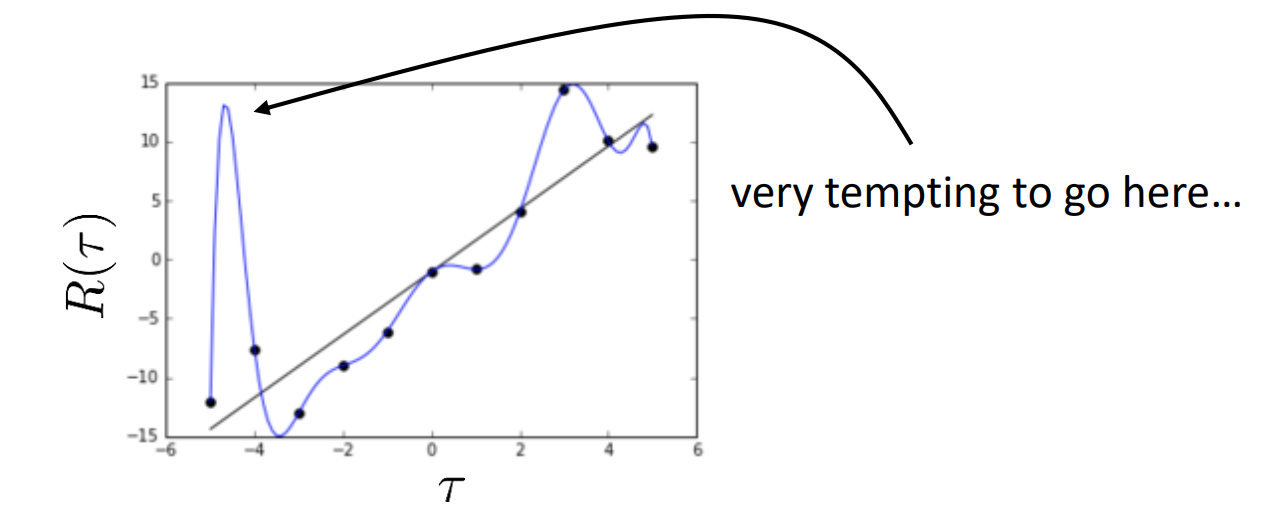
\includegraphics[scale=0.5]{figures/overfit.png}
    \caption{False belief about the model from overfitting}
    \label{fig:overfit}
\end{figure}

Therefore, we need to explore to get better, more representative data of the model, thus preventing overfitting and false belief. The expected value of the reward is not the same as optimistic or pessimistic. In step 5, when we choose actions, we only take actions for which we think we will get high reward in expectation, with respect to uncertain dynamics, which avoids exploiting the model too much.

\subsection{Uncertainty-aware Models}
Under imperfect models and model mismatch, one might expect wrong actions planned. Therefore, one way to deal with this problem is to construct an uncertainty-aware model, where we can quantitatively estimate the uncertainty in the model, so that we can assess the accuracy of the model and the planned actions. 

The first idea is to use entropy of output distribution, and as we know, higher entropy means higher uncertainty. We can estimate the entropy of $p(s_{t+1}|s_t,a_t)$. However, this is not enough because when the model is wrong, we might still have low variance, thus low entropy. Even though in some regions the model is highly uncertain, the output entropy is still low.

The reason why entropy of the output distribution alone is not expressive enough is that there are two types of uncertainty:
\begin{itemize}
    \item aleatoric (statistical) uncertainty, where the data itself is noisy.
    \item epistemic (model) uncertainty, where the model is certain about data, but we are not certain about model.
\end{itemize}
These two types of uncertainty are not the same. We cannot gauge the correctness of the second model based on the output entropy, and the entropy of the first model might be higher even though it is potentially a very ``good'' model. 

The second idea is to estimate the model uncertainty, where we essentially estimate how uncertainty we are about the model.
\begin{figure}
    \centering
    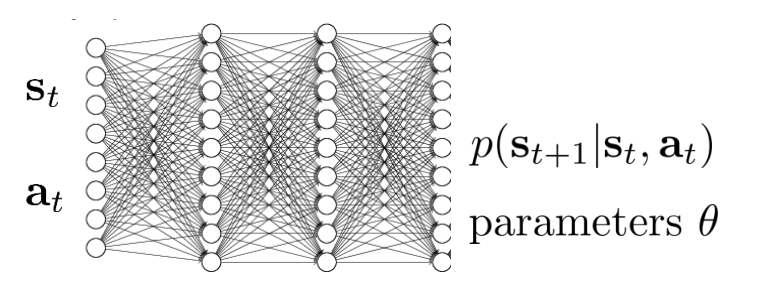
\includegraphics[scale=0.5]{figures/modelnn.png}
    \caption{Estimating the model using a neural net}
    \label{fig:modelnn}
\end{figure}
Usually, we use maximum likelihood estimation, where
\[
\argmaxA_\theta \log p(\theta|\mathcal{D}) = \argmaxA_\theta \log p(\mathcal{D}|\theta)
\]
Instead if we estimate the posterior of data $p(\theta|\mathcal{D})$ instead of argmax, the entropy of the distribution gives us the model uncertainty from the data. Moreover, we can predict using $\int p(s_{t+1}|s_t,a_t,\theta)p(\theta|\mathcal{D}) d\theta$.

To learn the posterior distribution, we can apply bootstrap ensembles, where we use multiple networks to learn the same distribution. Formally, say we have $N$ networks, each with a parameter $\theta_i$ to learn $p(s_{t+1}|s_t,a_t)$, we can then estimate the posterior by:
\[
p(\theta|\mathcal{D}) \simeq \frac{1}{N}\sum_i \delta(\theta_i)
\]
where $\delta(\cdot)$ is the direc-delta function. To train it, we need to generate independent datasets to get independent models. One way to do this is to train $\theta_i$ on $\mathcal{D}_i$ sampled with replacement from $\mathcal{D}$. This method is simple, but it is a very crude approximation. 

With this ensemble of networks, we choose actions a little differently. Before, we choose actions by $J(a_1,\dots,a_H) = \sum_{t=1}^Hr(s_t,a_t)$, where $s_{t+1} = f(s_t,a_t)$, and now we average over the ensemble by $J(a_1,\dots,a_H) = \frac{1}{N}\sum_{i=1}^N\sum_{t=1}^Hr(s_{t,i},a_{t,i})$, where $s_{t+1,i} = f(s_{t,i},a_{t,i})$

In general, for candidate action sequence $a_1,\dots,a_H$, we first sample $\theta \sim p(\theta|\mathcal{D})$, then at each time step $t$, we sample $s_{t+1}\sim p(s_{t+1}|s_t,a_t,\theta)$, then we calculate the reward $R = \sum_t r(s_t,a_t)$, and we repeat the aforementioned steps and accumulate the average reward.
% idk how this works....
\subsection{Latent Space Model}
In many cases, we are given very complex observations of the states such as pixel-based images, where we do not have full access to the states. To learn the dynamics using observations, we need to learn from the latent space and infer the states from observations. 
\begin{figure}
    \centering
    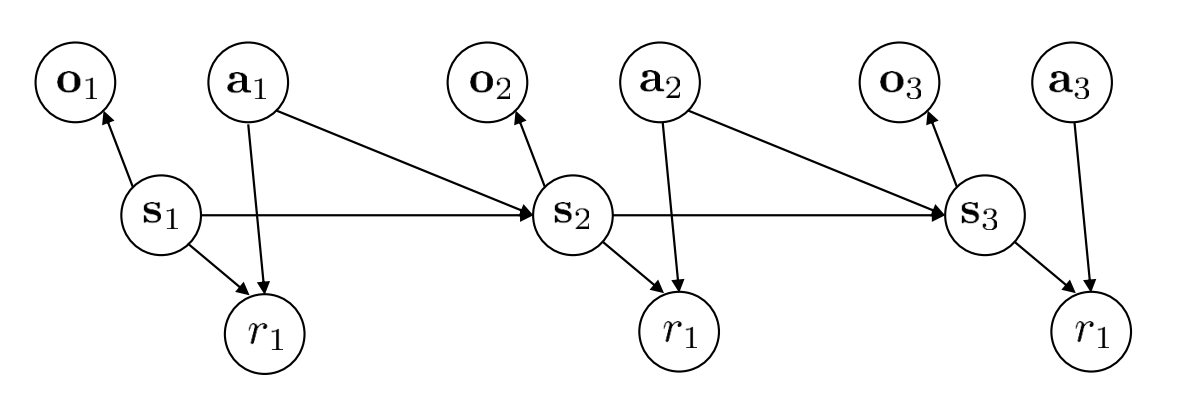
\includegraphics[scale=0.4]{figures/latent.png}
    \caption{Latent space model}
    \label{fig:latent}
\end{figure}
From Fig. \ref{fig:latent}, we can see that we need to learn the following models:
\begin{itemize}
    \item $p(o_t|s_t)$, the observation model
    \item $p(s_{t+1}|s_t,a_t)$, the dynamics model
    \item $p(r_t|s_t,a_t)$, the reward model
\end{itemize}

Recall that in high level, model-based RL algorithms are basically doing a maximum likelihood estimation in training given fully observed states:
\[
\max_\phi \frac{1}{N}\sum_{i=1}^N\sum_{t=1}^T\log p_\phi(s_{t+1,i}|s_{t,i},a_{t,i})
\]
then with latent models, we are not sure about the actual state, so we take the expected value:
\[
\max_\phi \frac{1}{N}\sum_{i=1}^N\sum_{t=1}^T\mathbb{E}\left[\log p_\phi(s_{t+1,i}|s_{t,i},a_{t,i}) + \log p_\phi(o_{t,i}|s_{t,i})\right]
\]
where the expectation is with respect to the distribution of $(s_t,s_{t+1})\sim p(s_t,s_{t+1}|o_{1:T},a_{1:T})$

However, the posterior distribution $p(s_t,s_{t+1}|o_{1:T},a_{1:T})$ is usually intractable if we have very complex dynamics. As a result, we could instead try to learn an approximate posterior, which we call $q_\psi(s_t|o_{1:t},a_{1;t})$. We could also learn $q_\psi(s_t,s_{t+1}|o_{1:t},a_{1;t})$ and $q_\psi(s_t|o_t)$. We call this technique learning an \textbf{encoder}. Learning the distribution $q_\psi(s_t|o_t)$ is crude, but it is the simplest to implement. If we just decide to learn this distribution for now, then the expectation becomes:
\[
\max_\phi \frac{1}{N}\sum_{i=1}^N\sum_{t=1}^T\mathbb{E}\left[\log p_\phi(s_{t+1,i}|s_{t,i},a_{t,i}) + \log p_\phi(o_{t,i}|s_{t,i})\right]
\]
such that the expectation is with respect to $s_t\sim q_\psi(s_t|o_t)$, $s_{t+1}\sim q_\psi(s_{t+1}|o_{t+1})$

For now, let us focus on a simple case where $q(s_t|o_t)$ is deterministic, because the stochastic requires variational inference, which will be covered in-depth in a later chapter. In deterministic case, we are training a neural net $g_\psi(o_t) = s_t$ using a direc-delta function such that $q_\psi(s_t|o_t) = \delta(s_t = g_\psi(o_t))$. Then the expectation can be simplified as
\[
\max_\phi \frac{1}{N}\sum_{i=1}^N\sum_{t=1}^T\log p_\phi(g_\psi(o_{t+1,i})|g_\psi(o_{t,i}),a_{t,i}) + \log p_\phi(o_{t,i}|g_\psi(o_{t,i}))
\]
Now everything is differentiable, we can train using backpropagation. 

Thus, we can slightly modify Alg. \ref{alg:mb15} so that we can deal with observations and latent space. We show the sketch of this slightly modified algorithm in Alg. \ref{alg:mblatent}. In step 4, we are respectively learning the dynamics, reward model, observation model, and encoder.
\begin{algorithm}[t!]
\caption{Model-based Reinforcement Learning with Latent States}
\begin{algorithmic}[1]
\label{alg:mblatent}
\REQUIRE Some base policy for data collection $\pi_0$, hyperparameter $N$
\STATE Run base policy $\pi(a_t|s_t)$ (e.g. random policy) to collect $\mathcal{D} = \{(s,a,s')_i\}$
\FOR{every $N$ steps}
\WHILE{True}
\STATE Learn dynamics model $p_\phi(s_{t+1}|s_t,a_t),p_\phi(r_t|s_t),p(o_t|s_t),g_\psi(o_t)$
\STATE Plan through $f(s,a)$ to choose actions
\STATE Execute the first planned action, observe resulting state $o'$ (MPC)
\STATE Append $(o,a,o')$ to dataset $\mathcal{D}$
\ENDWHILE
\ENDFOR
\end{algorithmic}
\end{algorithm}

Interested readers can refer to \cite{watter2015embed} and \cite{zhang2018solar} for more information on learning from pixel-based images as latent states.